\subsection{Цель выполнения домашнего задания}\label{blockN.VariantM}
\textbf{Цель выполнения домашнего задания }-- \GoalOfResearch

%-------------------------------------------------
\subsection{Задание}
Рассматривается система, аналогичная задаче $№3$, но в которой возможна организация ремонта ранее вышедших из строя устройств.
Одновременно может ремонтироваться только одно устройство.
Если подлежат ремонту устройства разных типов, приоритет отдаётся тем, которых сломалось больше,
а если их сломалось одинаковое число – тому типу, интенсивность поломок которого выше.
Интенсивность ремонта устройств обоих типов одинакова и равна $\lambda_S = (N_A + N_B - (G \bmod 3)) * (G + (N \bmod 4))$.


Если $N$ – номер зачётной книжки, а $G$ – последняя цифра в номере группы,
то параметры системы определяются следующим образом:
\[
\begin{matrix}
    \lambda_A= G + (N \bmod 3) \\
    \lambda_B= G + (N \bmod 5) \\
    N_A= 2 + (G \bmod 2) \\
    N_B= 2 + (N \bmod 2) \\
    R_A= 4 + (G \bmod 2) \\
    R_B= 5 - (G \bmod 2) \\
    \lambda_S = (N_A + N_B - (G \bmod 3)) * (G + (N \bmod 4))
\end{matrix}
\]

Требуется:
\begin{enumerate}
    \item нарисовать граф состояний системы;
    \item составить матрицу интенсивностей переходов;
    \item записать алгебраические уравнения Колмогорова для установившегося режима работы;
    \item рассчитать предельные вероятности состояний системы;
    \item рассчитать математические ожидания прикладных характеристик системы:
    \begin{itemize}
        \item вероятности отказа системы;
        \item числа готовых к эксплуатации устройств каждого типа;
        \item коэффициента загрузки ремонтной службы.
    \end{itemize}
    \item записать дифференциальные уравнения Колмогорова;
    \item методами численного интегрирования решить полученную систему уравнений, исходя из того, что в начальный момент времени все устройства исправны, а время моделирования выбирается вдвое больше теоретической оценки времени переходного процесса (т.е. того времени, которое необходимо, чтобы эвклидова норма вектора невязки с ранее рассчитанным предельным вектором составляла не более 10\% эвклидовой нормы последнего);
    \item построить графики вероятностей нахождения системы в каждом из возможных состояний с течением времени;
    \item провести имитационное моделирование системы в терминах непрерывных марковских цепей 100 раз, время моделирования выбирается вдвое больше экспериментальной оценки времени переходного процесса (т.е. того времени, которое необходимо, чтобы накопленная доля времени пребывания системы в каждом из состояний отличалась не более чем на 10\% от результатов, полученных при обработке предыдущего переключения цепи), проанализировать статистику времени выхода на установившийся режим работы и рассчитать статистические оценки предельных вероятностей после выхода на установившийся режим;
    \item провести имитационное моделирование системы в терминах дискретно-событийного моделирования (с независимым планированием времени наступления событий для каждого устройства в отдельности) 100 раз, время моделирования выбирается вдвое больше экспериментальной оценки времени переходного процесса (т.е. того времени, которое необходимо, чтобы накопленные средние оценки прикладных характеристик системы отличалась не более чем на 10\% от результатов, полученных при обработке предыдущего события в системе), проанализировать статистику времени выхода на установившийся режим работы и рассчитать статистические оценки для прикладных характеристик системы после выхода на установившийся режим.
\end{enumerate}
%-------------------------------------------------
\newpage
\subsection{Решение}

Рассчитаем начальные данные для выполнения домашнего задания по номеру зачетки $N = 169$ и группы $G = 5$:
\[
\begin{matrix}
    \lambda_A & = G + (N \bmod 3) = 5 + (169 \bmod 3) = & 6 \\
    \lambda_B & = G + (N \bmod 5) = 5 + (169 \bmod 5) = & 9 \\
    N_A & = 2 + (G \bmod 2) = 2 + (5 \bmod 2) = & 3 \\
    N_B & = 2 + (N \bmod 2) = 2 + (169 \bmod 2) = & 3 \\
    R_A & = 4 + (G \bmod 2) = 4 + (5 \bmod 2) = & 5 \\
    R_B & = 5 - (G \bmod 2) = 5 - (5 \bmod 2) = & 4 \\
    \lambda_S & = (N_A + N_B - (G \bmod 3)) * (G + (N \bmod 4)) = & 24
\end{matrix}
\]

Предположим что $S^{ab}_{cd}$ - состояние системы, где
\begin{itemize}
    \item $a$ - количество работающих устройств типа $A$,
    \item $b$ - количество резервных устройств типа $A$,
    \item $c$ - количество работающих устройств типа $B$,
    \item $d$ - количество резервных устройств типа $B$.
\end{itemize}
На рисунке \ref{graph} изображен граф состояний системы.

Для системы с данными параметрами был получен граф состояний системы, представленный на рисунке \ref{graph}. Верхние и нижние индексы -- пара чисел, первое -- рабочие устройства типа $А$ (верхний) или $В$ (нижний), второе -- остаток в резерве.

\begin{figure}[H]

    \centerline{
        \resizebox{10cm}{!}{
                
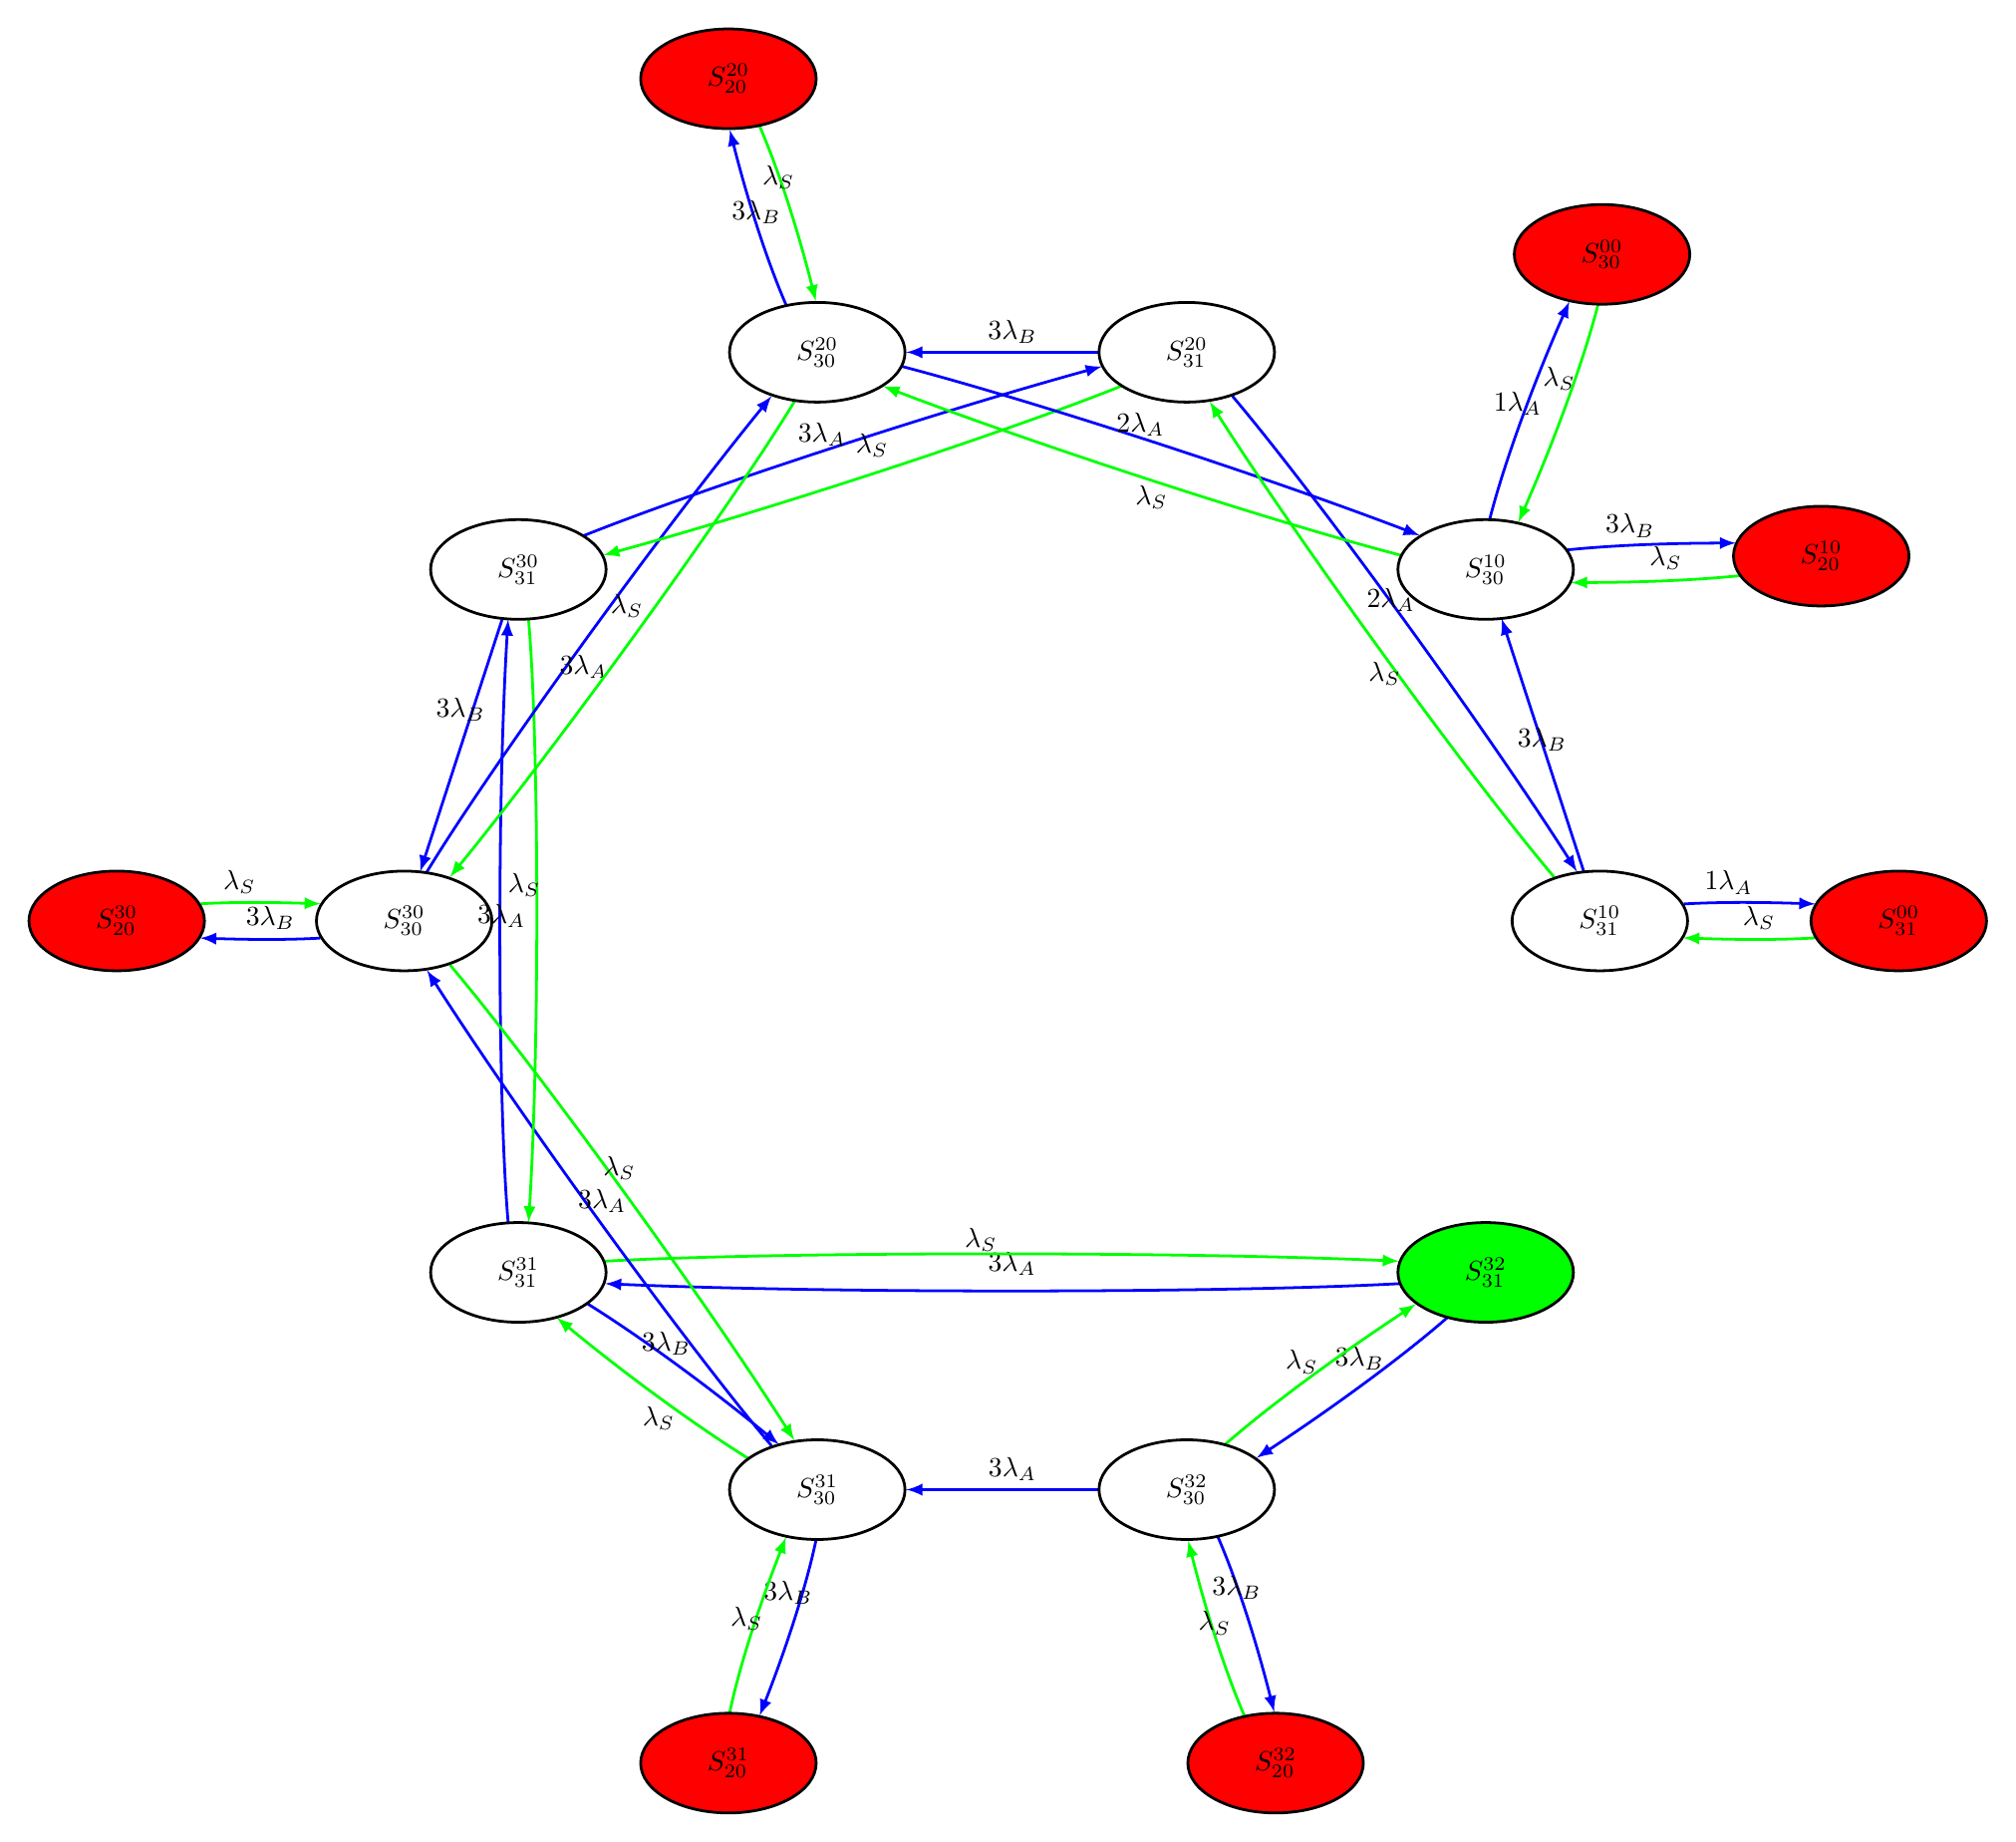
\begin{tikzpicture}[>=latex,line join=bevel,]
  \pgfsetlinewidth{1bp}
%%
\pgfsetcolor{black}
  % Edge: s3231 -> s3230
  \pgfsetcolor{blue}
  \draw [->] (512.48bp,178.86bp) .. controls (497.52bp,165.8bp) and (473.3bp,147.74bp)  .. (443.65bp,128.24bp);
  \definecolor{strokecol}{rgb}{0.0,0.0,0.0};
  \pgfsetstrokecolor{strokecol}
  \draw (480.82bp,164.12bp) node {$3\lambda_B$};
  % Edge: s3231 -> s3131
  \pgfsetcolor{blue}
  \draw [->] (495.06bp,191.15bp) .. controls (432.22bp,187.76bp) and (290.7bp,187.58bp)  .. (208.31bp,191.15bp);
  \definecolor{strokecol}{rgb}{0.0,0.0,0.0};
  \pgfsetstrokecolor{strokecol}
  \draw (355.29bp,198.38bp) node {$3\lambda_A$};
  % Edge: s3230 -> s3231
  \pgfsetcolor{green}
  \draw [->] (432.29bp,133.12bp) .. controls (447.25bp,146.19bp) and (471.48bp,164.25bp)  .. (501.13bp,183.75bp);
  \definecolor{strokecol}{rgb}{0.0,0.0,0.0};
  \pgfsetstrokecolor{strokecol}
  \draw (459.96bp,162.86bp) node {$\lambda_S$};
  % Edge: s3230 -> s3220
  \pgfsetcolor{blue}
  \draw [->] (429.58bp,99.86bp) .. controls (435.81bp,85.522bp) and (442.85bp,64.649bp)  .. (449.98bp,36.462bp);
  \definecolor{strokecol}{rgb}{0.0,0.0,0.0};
  \pgfsetstrokecolor{strokecol}
  \draw (436.45bp,81.21bp) node {$3\lambda_B$};
  % Edge: s3230 -> s3130
  \pgfsetcolor{blue}
  \draw [->] (386.43bp,116.76bp) .. controls (369.05bp,116.76bp) and (347.32bp,116.76bp)  .. (317.09bp,116.76bp);
  \definecolor{strokecol}{rgb}{0.0,0.0,0.0};
  \pgfsetstrokecolor{strokecol}
  \draw (355.43bp,124.26bp) node {$3\lambda_A$};
  % Edge: s3131 -> s3231
  \pgfsetcolor{green}
  \draw [->] (208.26bp,199.28bp) .. controls (271.1bp,202.67bp) and (412.62bp,202.85bp)  .. (495.0bp,199.28bp);
  \definecolor{strokecol}{rgb}{0.0,0.0,0.0};
  \pgfsetstrokecolor{strokecol}
  \draw (344.03bp,207.05bp) node {$\lambda_S$};
  % Edge: s3131 -> s3130
  \pgfsetcolor{blue}
  \draw [->] (202.05bp,183.83bp) .. controls (220.35bp,172.38bp) and (244.86bp,154.7bp)  .. (271.03bp,133.11bp);
  \definecolor{strokecol}{rgb}{0.0,0.0,0.0};
  \pgfsetstrokecolor{strokecol}
  \draw (230.28bp,169.56bp) node {$3\lambda_B$};
  % Edge: s3131 -> s3031
  \pgfsetcolor{blue}
  \draw [->] (173.24bp,213.48bp) .. controls (169.46bp,256.93bp) and (169.19bp,366.82bp)  .. (173.25bp,431.01bp);
  \definecolor{strokecol}{rgb}{0.0,0.0,0.0};
  \pgfsetstrokecolor{strokecol}
  \draw (170.83bp,324.11bp) node {$3\lambda_A$};
  % Edge: s3220 -> s3230
  \pgfsetcolor{green}
  \draw [->] (439.3bp,34.905bp) .. controls (433.07bp,49.242bp) and (426.03bp,70.116bp)  .. (418.9bp,98.302bp);
  \definecolor{strokecol}{rgb}{0.0,0.0,0.0};
  \pgfsetstrokecolor{strokecol}
  \draw (428.43bp,68.554bp) node {$\lambda_S$};
  % Edge: s3130 -> s3131
  \pgfsetcolor{green}
  \draw [->] (259.81bp,128.15bp) .. controls (241.51bp,139.6bp) and (217.01bp,157.28bp)  .. (190.83bp,178.87bp);
  \definecolor{strokecol}{rgb}{0.0,0.0,0.0};
  \pgfsetstrokecolor{strokecol}
  \draw (227.59bp,142.42bp) node {$\lambda_S$};
  % Edge: s3130 -> s3120
  \pgfsetcolor{blue}
  \draw [->] (284.44bp,98.398bp) .. controls (281.31bp,83.543bp) and (274.8bp,62.422bp)  .. (264.13bp,35.181bp);
  \definecolor{strokecol}{rgb}{0.0,0.0,0.0};
  \pgfsetstrokecolor{strokecol}
  \draw (274.39bp,79.473bp) node {$3\lambda_B$};
  % Edge: s3130 -> s3030
  \pgfsetcolor{blue}
  \draw [->] (268.4bp,132.61bp) .. controls (238.83bp,167.51bp) and (177.95bp,250.99bp)  .. (143.97bp,304.31bp);
  \definecolor{strokecol}{rgb}{0.0,0.0,0.0};
  \pgfsetstrokecolor{strokecol}
  \draw (207.21bp,221.12bp) node {$3\lambda_A$};
  % Edge: s3031 -> s3131
  \pgfsetcolor{green}
  \draw [->] (180.64bp,430.84bp) .. controls (184.42bp,387.38bp) and (184.68bp,277.49bp)  .. (180.63bp,213.31bp);
  \definecolor{strokecol}{rgb}{0.0,0.0,0.0};
  \pgfsetstrokecolor{strokecol}
  \draw (179.05bp,335.21bp) node {$\lambda_S$};
  % Edge: s3031 -> s3030
  \pgfsetcolor{blue}
  \draw [->] (171.12bp,431.18bp) .. controls (164.33bp,410.3bp) and (153.03bp,375.5bp)  .. (141.49bp,339.99bp);
  \definecolor{strokecol}{rgb}{0.0,0.0,0.0};
  \pgfsetstrokecolor{strokecol}
  \draw (156.07bp,398.51bp) node {$3\lambda_B$};
  % Edge: s3031 -> s2031
  \pgfsetcolor{blue}
  \draw [->] (200.54bp,461.3bp) .. controls (241.42bp,477.67bp) and (325.84bp,505.4bp)  .. (387.7bp,522.41bp);
  \definecolor{strokecol}{rgb}{0.0,0.0,0.0};
  \pgfsetstrokecolor{strokecol}
  \draw (286.65bp,497.88bp) node {$3\lambda_A$};
  % Edge: s3120 -> s3130
  \pgfsetcolor{green}
  \draw [->] (253.31bp,36.366bp) .. controls (256.44bp,51.221bp) and (262.95bp,72.342bp)  .. (273.62bp,99.583bp);
  \definecolor{strokecol}{rgb}{0.0,0.0,0.0};
  \pgfsetstrokecolor{strokecol}
  \draw (259.36bp,70.291bp) node {$\lambda_S$};
  % Edge: s3030 -> s3130
  \pgfsetcolor{green}
  \draw [->] (152.21bp,306.31bp) .. controls (181.78bp,271.41bp) and (242.66bp,187.93bp)  .. (276.64bp,134.61bp);
  \definecolor{strokecol}{rgb}{0.0,0.0,0.0};
  \pgfsetstrokecolor{strokecol}
  \draw (213.4bp,232.8bp) node {$\lambda_S$};
  % Edge: s3030 -> s3020
  \pgfsetcolor{blue}
  \draw [->] (105.38bp,315.96bp) .. controls (95.354bp,315.42bp) and (84.023bp,315.28bp)  .. (62.021bp,315.97bp);
  \definecolor{strokecol}{rgb}{0.0,0.0,0.0};
  \pgfsetstrokecolor{strokecol}
  \draw (87.344bp,323.24bp) node {$3\lambda_B$};
  % Edge: s3030 -> s2030
  \pgfsetcolor{blue}
  \draw [->] (143.86bp,339.81bp) .. controls (166.09bp,376.54bp) and (226.97bp,460.9bp)  .. (268.4bp,511.7bp);
  \definecolor{strokecol}{rgb}{0.0,0.0,0.0};
  \pgfsetstrokecolor{strokecol}
  \draw (200.5bp,413.87bp) node {$3\lambda_A$};
  % Edge: s2031 -> s3031
  \pgfsetcolor{green}
  \draw [->] (394.8bp,515.36bp) .. controls (353.92bp,498.99bp) and (269.5bp,471.25bp)  .. (207.63bp,454.24bp);
  \definecolor{strokecol}{rgb}{0.0,0.0,0.0};
  \pgfsetstrokecolor{strokecol}
  \draw (304.69bp,493.77bp) node {$\lambda_S$};
  % Edge: s2031 -> s2030
  \pgfsetcolor{blue}
  \draw [->] (386.43bp,527.55bp) .. controls (369.05bp,527.55bp) and (347.32bp,527.55bp)  .. (317.09bp,527.55bp);
  \definecolor{strokecol}{rgb}{0.0,0.0,0.0};
  \pgfsetstrokecolor{strokecol}
  \draw (355.43bp,535.05bp) node {$3\lambda_B$};
  % Edge: s2031 -> s1031
  \pgfsetcolor{blue}
  \draw [->] (434.91bp,511.7bp) .. controls (464.48bp,476.81bp) and (525.36bp,393.32bp)  .. (559.34bp,340.01bp);
  \definecolor{strokecol}{rgb}{0.0,0.0,0.0};
  \pgfsetstrokecolor{strokecol}
  \draw (492.1bp,438.2bp) node {$2\lambda_A$};
  % Edge: s3020 -> s3030
  \pgfsetcolor{green}
  \draw [->] (62.163bp,328.36bp) .. controls (72.187bp,328.9bp) and (83.519bp,329.04bp)  .. (105.52bp,328.35bp);
  \definecolor{strokecol}{rgb}{0.0,0.0,0.0};
  \pgfsetstrokecolor{strokecol}
  \draw (76.197bp,336.07bp) node {$\lambda_S$};
  % Edge: s2030 -> s3030
  \pgfsetcolor{green}
  \draw [->] (276.76bp,509.9bp) .. controls (254.53bp,473.17bp) and (193.65bp,388.81bp)  .. (152.22bp,338.01bp);
  \definecolor{strokecol}{rgb}{0.0,0.0,0.0};
  \pgfsetstrokecolor{strokecol}
  \draw (216.12bp,435.84bp) node {$\lambda_S$};
  % Edge: s2030 -> s2020
  \pgfsetcolor{blue}
  \draw [->] (273.74bp,544.46bp) .. controls (267.51bp,558.8bp) and (260.47bp,579.67bp)  .. (253.33bp,607.86bp);
  \definecolor{strokecol}{rgb}{0.0,0.0,0.0};
  \pgfsetstrokecolor{strokecol}
  \draw (262.86bp,578.11bp) node {$3\lambda_B$};
  % Edge: s2030 -> s1030
  \pgfsetcolor{blue}
  \draw [->] (315.46bp,522.45bp) .. controls (360.56bp,510.69bp) and (444.65bp,483.5bp)  .. (502.51bp,461.4bp);
  \definecolor{strokecol}{rgb}{0.0,0.0,0.0};
  \pgfsetstrokecolor{strokecol}
  \draw (401.68bp,501.49bp) node {$2\lambda_A$};
  % Edge: s1031 -> s2031
  \pgfsetcolor{green}
  \draw [->] (551.11bp,338.01bp) .. controls (521.53bp,372.9bp) and (460.66bp,456.39bp)  .. (426.68bp,509.7bp);
  \definecolor{strokecol}{rgb}{0.0,0.0,0.0};
  \pgfsetstrokecolor{strokecol}
  \draw (489.92bp,411.52bp) node {$\lambda_S$};
  % Edge: s1031 -> s1030
  \pgfsetcolor{blue}
  \draw [->] (561.8bp,340.08bp) .. controls (555.01bp,360.96bp) and (543.71bp,395.76bp)  .. (532.17bp,431.27bp);
  \definecolor{strokecol}{rgb}{0.0,0.0,0.0};
  \pgfsetstrokecolor{strokecol}
  \draw (546.75bp,387.75bp) node {$3\lambda_B$};
  % Edge: s1031 -> s0031
  \pgfsetcolor{blue}
  \draw [->] (597.99bp,328.3bp) .. controls (609.24bp,328.92bp) and (622.2bp,329.07bp)  .. (645.47bp,328.29bp);
  \definecolor{strokecol}{rgb}{0.0,0.0,0.0};
  \pgfsetstrokecolor{strokecol}
  \draw (614.12bp,336.02bp) node {$1\lambda_A$};
  % Edge: s2020 -> s2030
  \pgfsetcolor{green}
  \draw [->] (264.01bp,609.41bp) .. controls (270.25bp,595.08bp) and (277.28bp,574.2bp)  .. (284.42bp,546.02bp);
  \definecolor{strokecol}{rgb}{0.0,0.0,0.0};
  \pgfsetstrokecolor{strokecol}
  \draw (270.89bp,590.76bp) node {$\lambda_S$};
  % Edge: s1030 -> s2030
  \pgfsetcolor{green}
  \draw [->] (495.84bp,454.2bp) .. controls (450.74bp,465.96bp) and (366.65bp,493.15bp)  .. (308.79bp,515.25bp);
  \definecolor{strokecol}{rgb}{0.0,0.0,0.0};
  \pgfsetstrokecolor{strokecol}
  \draw (405.62bp,475.16bp) node {$\lambda_S$};
  % Edge: s1030 -> s1020
  \pgfsetcolor{blue}
  \draw [->] (555.8bp,456.17bp) .. controls (570.65bp,457.66bp) and (588.94bp,458.58bp)  .. (616.75bp,458.65bp);
  \definecolor{strokecol}{rgb}{0.0,0.0,0.0};
  \pgfsetstrokecolor{strokecol}
  \draw (578.54bp,464.94bp) node {$3\lambda_B$};
  % Edge: s1030 -> s0030
  \pgfsetcolor{blue}
  \draw [->] (527.87bp,467.35bp) .. controls (532.55bp,485.79bp) and (542.76bp,514.44bp)  .. (556.61bp,545.85bp);
  \definecolor{strokecol}{rgb}{0.0,0.0,0.0};
  \pgfsetstrokecolor{strokecol}
  \draw (537.9bp,508.96bp) node {$1\lambda_A$};
  % Edge: s0031 -> s1031
  \pgfsetcolor{green}
  \draw [->] (645.24bp,316.02bp) .. controls (633.99bp,315.4bp) and (621.03bp,315.25bp)  .. (597.76bp,316.03bp);
  \definecolor{strokecol}{rgb}{0.0,0.0,0.0};
  \pgfsetstrokecolor{strokecol}
  \draw (625.1bp,323.3bp) node {$\lambda_S$};
  % Edge: s1020 -> s1030
  \pgfsetcolor{green}
  \draw [->] (618.18bp,446.85bp) .. controls (603.32bp,445.36bp) and (585.03bp,444.44bp)  .. (557.23bp,444.37bp);
  \definecolor{strokecol}{rgb}{0.0,0.0,0.0};
  \pgfsetstrokecolor{strokecol}
  \draw (591.44bp,453.08bp) node {$\lambda_S$};
  % Edge: s0030 -> s1030
  \pgfsetcolor{green}
  \draw [->] (566.93bp,544.64bp) .. controls (562.25bp,526.21bp) and (552.04bp,497.56bp)  .. (538.19bp,466.15bp);
  \definecolor{strokecol}{rgb}{0.0,0.0,0.0};
  \pgfsetstrokecolor{strokecol}
  \draw (552.9bp,518.03bp) node {$\lambda_S$};
  % Node: s3231
\begin{scope}
  \definecolor{strokecol}{rgb}{0.0,0.0,0.0};
  \pgfsetstrokecolor{strokecol}
  \definecolor{fillcol}{rgb}{0.0,1.0,0.0};
  \pgfsetfillcolor{fillcol}
  \filldraw [opacity=1] (526.38bp,195.22bp) ellipse (31.7bp and 18.0bp);
  \draw (526.38bp,195.22bp) node {$S^{32}_{31}$};
\end{scope}
  % Node: s3230
\begin{scope}
  \definecolor{strokecol}{rgb}{0.0,0.0,0.0};
  \pgfsetstrokecolor{strokecol}
  \draw (418.4bp,116.76bp) ellipse (31.7bp and 18.0bp);
  \draw (418.4bp,116.76bp) node {$S^{32}_{30}$};
\end{scope}
  % Node: s3131
\begin{scope}
  \definecolor{strokecol}{rgb}{0.0,0.0,0.0};
  \pgfsetstrokecolor{strokecol}
  \draw (176.94bp,195.22bp) ellipse (31.7bp and 18.0bp);
  \draw (176.94bp,195.22bp) node {$S^{31}_{31}$};
\end{scope}
  % Node: s3220
\begin{scope}
  \definecolor{strokecol}{rgb}{0.0,0.0,0.0};
  \pgfsetstrokecolor{strokecol}
  \definecolor{fillcol}{rgb}{1.0,0.0,0.0};
  \pgfsetfillcolor{fillcol}
  \filldraw [opacity=1] (450.49bp,18.0bp) ellipse (31.7bp and 18.0bp);
  \draw (450.49bp,18.0bp) node {$S^{32}_{20}$};
\end{scope}
  % Node: s3130
\begin{scope}
  \definecolor{strokecol}{rgb}{0.0,0.0,0.0};
  \pgfsetstrokecolor{strokecol}
  \draw (284.92bp,116.76bp) ellipse (31.7bp and 18.0bp);
  \draw (284.92bp,116.76bp) node {$S^{31}_{30}$};
\end{scope}
  % Node: s3031
\begin{scope}
  \definecolor{strokecol}{rgb}{0.0,0.0,0.0};
  \pgfsetstrokecolor{strokecol}
  \draw (176.94bp,449.1bp) ellipse (31.7bp and 18.0bp);
  \draw (176.94bp,449.1bp) node {$S^{30}_{31}$};
\end{scope}
  % Node: s3120
\begin{scope}
  \definecolor{strokecol}{rgb}{0.0,0.0,0.0};
  \pgfsetstrokecolor{strokecol}
  \definecolor{fillcol}{rgb}{1.0,0.0,0.0};
  \pgfsetfillcolor{fillcol}
  \filldraw [opacity=1] (252.83bp,18.0bp) ellipse (31.7bp and 18.0bp);
  \draw (252.83bp,18.0bp) node {$S^{31}_{20}$};
\end{scope}
  % Node: s3030
\begin{scope}
  \definecolor{strokecol}{rgb}{0.0,0.0,0.0};
  \pgfsetstrokecolor{strokecol}
  \draw (135.69bp,322.16bp) ellipse (31.7bp and 18.0bp);
  \draw (135.69bp,322.16bp) node {$S^{30}_{30}$};
\end{scope}
  % Node: s2031
\begin{scope}
  \definecolor{strokecol}{rgb}{0.0,0.0,0.0};
  \pgfsetstrokecolor{strokecol}
  \draw (418.4bp,527.55bp) ellipse (31.7bp and 18.0bp);
  \draw (418.4bp,527.55bp) node {$S^{20}_{31}$};
\end{scope}
  % Node: s3020
\begin{scope}
  \definecolor{strokecol}{rgb}{0.0,0.0,0.0};
  \pgfsetstrokecolor{strokecol}
  \definecolor{fillcol}{rgb}{1.0,0.0,0.0};
  \pgfsetfillcolor{fillcol}
  \filldraw [opacity=1] (31.85bp,322.16bp) ellipse (31.7bp and 18.0bp);
  \draw (31.847bp,322.16bp) node {$S^{30}_{20}$};
\end{scope}
  % Node: s2030
\begin{scope}
  \definecolor{strokecol}{rgb}{0.0,0.0,0.0};
  \pgfsetstrokecolor{strokecol}
  \draw (284.92bp,527.55bp) ellipse (31.7bp and 18.0bp);
  \draw (284.92bp,527.55bp) node {$S^{20}_{30}$};
\end{scope}
  % Node: s1031
\begin{scope}
  \definecolor{strokecol}{rgb}{0.0,0.0,0.0};
  \pgfsetstrokecolor{strokecol}
  \draw (567.62bp,322.16bp) ellipse (31.7bp and 18.0bp);
  \draw (567.62bp,322.16bp) node {$S^{10}_{31}$};
\end{scope}
  % Node: s2020
\begin{scope}
  \definecolor{strokecol}{rgb}{0.0,0.0,0.0};
  \pgfsetstrokecolor{strokecol}
  \definecolor{fillcol}{rgb}{1.0,0.0,0.0};
  \pgfsetfillcolor{fillcol}
  \filldraw [opacity=1] (252.83bp,626.32bp) ellipse (31.7bp and 18.0bp);
  \draw (252.83bp,626.32bp) node {$S^{20}_{20}$};
\end{scope}
  % Node: s1030
\begin{scope}
  \definecolor{strokecol}{rgb}{0.0,0.0,0.0};
  \pgfsetstrokecolor{strokecol}
  \draw (526.38bp,449.1bp) ellipse (31.7bp and 18.0bp);
  \draw (526.38bp,449.1bp) node {$S^{10}_{30}$};
\end{scope}
  % Node: s0031
\begin{scope}
  \definecolor{strokecol}{rgb}{0.0,0.0,0.0};
  \pgfsetstrokecolor{strokecol}
  \definecolor{fillcol}{rgb}{1.0,0.0,0.0};
  \pgfsetfillcolor{fillcol}
  \filldraw [opacity=1] (675.61bp,322.16bp) ellipse (31.7bp and 18.0bp);
  \draw (675.61bp,322.16bp) node {$S^{00}_{31}$};
\end{scope}
  % Node: s1020
\begin{scope}
  \definecolor{strokecol}{rgb}{0.0,0.0,0.0};
  \pgfsetstrokecolor{strokecol}
  \definecolor{fillcol}{rgb}{1.0,0.0,0.0};
  \pgfsetfillcolor{fillcol}
  \filldraw [opacity=1] (647.6bp,453.92bp) ellipse (31.7bp and 18.0bp);
  \draw (647.6bp,453.92bp) node {$S^{10}_{20}$};
\end{scope}
  % Node: s0030
\begin{scope}
  \definecolor{strokecol}{rgb}{0.0,0.0,0.0};
  \pgfsetstrokecolor{strokecol}
  \definecolor{fillcol}{rgb}{1.0,0.0,0.0};
  \pgfsetfillcolor{fillcol}
  \filldraw [opacity=1] (568.42bp,562.9bp) ellipse (31.7bp and 18.0bp);
  \draw (568.42bp,562.9bp) node {$S^{00}_{30}$};
\end{scope}
%
\end{tikzpicture}

        }
    }

    \caption{Граф состояний системы ($\lambda_A = 6$, $\lambda_B = 9$)}
    \label{graph}
\end{figure}

По данному графу была получена матрица интенсивности:

\[
    \resizebox{\textwidth}{!}{$
        \Lambda =
        \begin{pmatrix}
        -45 & 27 & 18 & 0 & 0 & 0 & 0 & 0 & 0 & 0 & 0 & 0 & 0 & 0 & 0 & 0 & 0 \\
24 & -69 & 0 & 27 & 18 & 0 & 0 & 0 & 0 & 0 & 0 & 0 & 0 & 0 & 0 & 0 & 0 \\
24 & 0 & -69 & 0 & 27 & 18 & 0 & 0 & 0 & 0 & 0 & 0 & 0 & 0 & 0 & 0 & 0 \\
0 & 24 & 0 & -24 & 0 & 0 & 0 & 0 & 0 & 0 & 0 & 0 & 0 & 0 & 0 & 0 & 0 \\
0 & 0 & 24 & 0 & -69 & 0 & 27 & 18 & 0 & 0 & 0 & 0 & 0 & 0 & 0 & 0 & 0 \\
0 & 0 & 24 & 0 & 0 & -69 & 0 & 27 & 18 & 0 & 0 & 0 & 0 & 0 & 0 & 0 & 0 \\
0 & 0 & 0 & 0 & 24 & 0 & -24 & 0 & 0 & 0 & 0 & 0 & 0 & 0 & 0 & 0 & 0 \\
0 & 0 & 0 & 0 & 24 & 0 & 0 & -69 & 0 & 27 & 18 & 0 & 0 & 0 & 0 & 0 & 0 \\
0 & 0 & 0 & 0 & 0 & 24 & 0 & 0 & -63 & 0 & 27 & 12 & 0 & 0 & 0 & 0 & 0 \\
0 & 0 & 0 & 0 & 0 & 0 & 0 & 24 & 0 & -24 & 0 & 0 & 0 & 0 & 0 & 0 & 0 \\
0 & 0 & 0 & 0 & 0 & 0 & 0 & 24 & 0 & 0 & -63 & 0 & 27 & 12 & 0 & 0 & 0 \\
0 & 0 & 0 & 0 & 0 & 0 & 0 & 0 & 24 & 0 & 0 & -57 & 0 & 27 & 6 & 0 & 0 \\
0 & 0 & 0 & 0 & 0 & 0 & 0 & 0 & 0 & 0 & 24 & 0 & -24 & 0 & 0 & 0 & 0 \\
0 & 0 & 0 & 0 & 0 & 0 & 0 & 0 & 0 & 0 & 24 & 0 & 0 & -57 & 0 & 27 & 6 \\
0 & 0 & 0 & 0 & 0 & 0 & 0 & 0 & 0 & 0 & 0 & 24 & 0 & 0 & -24 & 0 & 0 \\
0 & 0 & 0 & 0 & 0 & 0 & 0 & 0 & 0 & 0 & 0 & 0 & 0 & 24 & 0 & -24 & 0 \\
0 & 0 & 0 & 0 & 0 & 0 & 0 & 0 & 0 & 0 & 0 & 0 & 0 & 24 & 0 & 0 & -24 
        \end{pmatrix}
    $}
\]

\subsection{Уравнения Колмогорова}
Составим систему алгебраических уравнений Колмогорова для установившегося режима работы.

\[
\begin{cases}
    0 = 24P_{1} (t) +24P_{2} (t) -27P_{0} (t) -18P_{0} (t) \\ 
0 = 27P_{0} (t) +24P_{3} (t) -24P_{1} (t) -27P_{1} (t) -18P_{1} (t) \\ 
0 = 18P_{0} (t) +24P_{4} (t) +24P_{5} (t) -24P_{2} (t) -27P_{2} (t) -18P_{2} (t) \\ 
0 = 27P_{1} (t) -24P_{3} (t) \\ 
0 = 18P_{1} (t) +27P_{2} (t) +24P_{6} (t) +24P_{7} (t) -24P_{4} (t) -27P_{4} (t) -18P_{4} (t) \\ 
0 = 18P_{2} (t) +24P_{8} (t) -24P_{5} (t) -27P_{5} (t) -18P_{5} (t) \\ 
0 = 27P_{4} (t) -24P_{6} (t) \\ 
0 = 18P_{4} (t) +27P_{5} (t) +24P_{9} (t) +24P_{10} (t) -24P_{7} (t) -27P_{7} (t) -18P_{7} (t) \\ 
0 = 18P_{5} (t) +24P_{11} (t) -24P_{8} (t) -27P_{8} (t) -12P_{8} (t) \\ 
0 = 27P_{7} (t) -24P_{9} (t) \\ 
0 = 18P_{7} (t) +27P_{8} (t) +24P_{12} (t) +24P_{13} (t) -24P_{10} (t) -27P_{10} (t) -12P_{10} (t) \\ 
0 = 12P_{8} (t) +24P_{14} (t) -24P_{11} (t) -27P_{11} (t) -6P_{11} (t) \\ 
0 = 27P_{10} (t) -24P_{12} (t) \\ 
0 = 12P_{10} (t) +27P_{11} (t) +24P_{15} (t) +24P_{16} (t) -24P_{13} (t) -27P_{13} (t) -6P_{13} (t) \\ 
0 = 6P_{11} (t) -24P_{14} (t) \\ 
0 = 27P_{13} (t) -24P_{15} (t) \\ 
0 = 6P_{13} (t) -24P_{16} (t) 
\end{cases}
\]

Условие нормировки: $\sum\limits_{i=0}^{ 16 }p_i=1$.
Тогда вектор предельных вероятностей может быть найдет после решения СЛАУ вида $$\mathbf{\Lambda}^T\bar{p}=\bar{b}.$$

 Вектор предельных вероятностей:
 \[
    \resizebox{\textwidth}{!}{$
    \bar{p}= \left(  0.05, 0.03, 0.06, 0.03, 0.12, 0.02, 0.13, 0.11, 0.01, 0.13, 0.09, 0.0, 0.1, 0.05, 0.0, 0.05, 0.01 \right)
    $}
\]

Составим систему дифференциальных уравнений Колмогорова.
\[
\begin{cases}
    P^\prime_{0} = 24P_{1} (t) +24P_{2} (t) -27P_{0} (t) -18P_{0} (t) \\ 
P^\prime_{1} = 27P_{0} (t) +24P_{3} (t) -24P_{1} (t) -27P_{1} (t) -18P_{1} (t) \\ 
P^\prime_{2} = 18P_{0} (t) +24P_{4} (t) +24P_{5} (t) -24P_{2} (t) -27P_{2} (t) -18P_{2} (t) \\ 
P^\prime_{3} = 27P_{1} (t) -24P_{3} (t) \\ 
P^\prime_{4} = 18P_{1} (t) +27P_{2} (t) +24P_{6} (t) +24P_{7} (t) -24P_{4} (t) -27P_{4} (t) -18P_{4} (t) \\ 
P^\prime_{5} = 18P_{2} (t) +24P_{8} (t) -24P_{5} (t) -27P_{5} (t) -18P_{5} (t) \\ 
P^\prime_{6} = 27P_{4} (t) -24P_{6} (t) \\ 
P^\prime_{7} = 18P_{4} (t) +27P_{5} (t) +24P_{9} (t) +24P_{10} (t) -24P_{7} (t) -27P_{7} (t) -18P_{7} (t) \\ 
P^\prime_{8} = 18P_{5} (t) +24P_{11} (t) -24P_{8} (t) -27P_{8} (t) -12P_{8} (t) \\ 
P^\prime_{9} = 27P_{7} (t) -24P_{9} (t) \\ 
P^\prime_{10} = 18P_{7} (t) +27P_{8} (t) +24P_{12} (t) +24P_{13} (t) -24P_{10} (t) -27P_{10} (t) -12P_{10} (t) \\ 
P^\prime_{11} = 12P_{8} (t) +24P_{14} (t) -24P_{11} (t) -27P_{11} (t) -6P_{11} (t) \\ 
P^\prime_{12} = 27P_{10} (t) -24P_{12} (t) \\ 
P^\prime_{13} = 12P_{10} (t) +27P_{11} (t) +24P_{15} (t) +24P_{16} (t) -24P_{13} (t) -27P_{13} (t) -6P_{13} (t) \\ 
P^\prime_{14} = 6P_{11} (t) -24P_{14} (t) \\ 
P^\prime_{15} = 27P_{13} (t) -24P_{15} (t) \\ 
P^\prime_{16} = 6P_{13} (t) -24P_{16} (t) 
\end{cases}
\]

Система дифференциальных уравнений была решена неявным методом Эйлера (см. листинг \ref{eler}).

\begin{lstlisting}[language=python, label=eler,caption={\textit{Неявный метод Эйлера}}]
def backward_euler(u0, tau, vec, Q_T):
    from scipy import optimize
    from scipy.spatial import distance
    t = [0]
    u = [[x for x in u0]]

    def Phi(z, v):
        return z - tau * (Q_T @ z) - v

    u.append(optimize.fsolve(Phi, u[-1], args=(u[-1])))
    t.append(t[-1] + tau)

    # интегрируем пока L2 норма вектора невязки с ранее рассчитанным предельным вектором составляла не более 10\% L2 нормы последнего
    while distance.euclidean(u[-1], vec) > 0.1 * np.linalg.norm(vec):
        u.append(optimize.fsolve(Phi, u[-1], args=(u[-1])))
        t.append(t[-1] + tau)

    for _ in range(int(t[-1] / tau)):
        u.append(optimize.fsolve(Phi, u[-1], args=(u[-2])))
        t.append(t[-1] + tau)

    return np.array(u), t
\end{lstlisting}

~\\

По вычисленным функциям были построены графики вероятностей нахождения системы в каждом из возможных состояний с течением времени
(рисунки \ref{P_o}, \ref{P_i}).
\begin{figure}[H]
\centerline{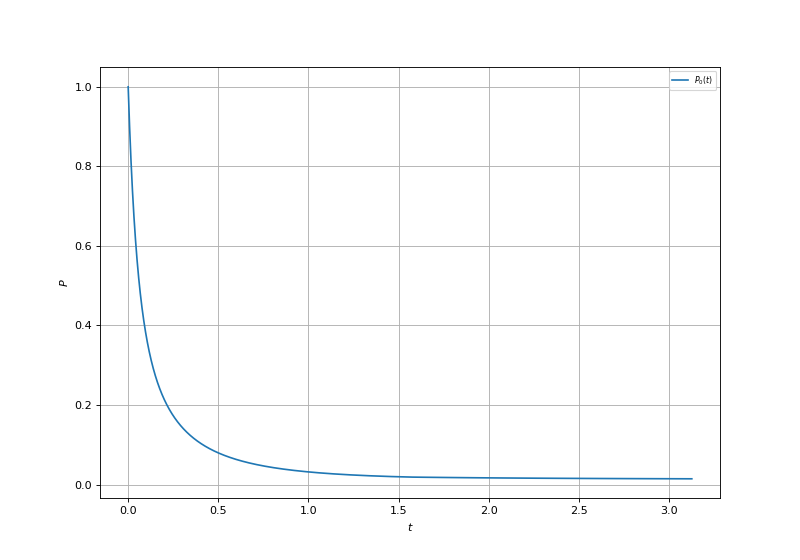
\includegraphics[width=\textwidth]{Images/P_o.png}}
\caption{Функция вероятности для 0 состояния}
\label{P_o}
\end{figure}

\begin{figure}[H]
\centerline{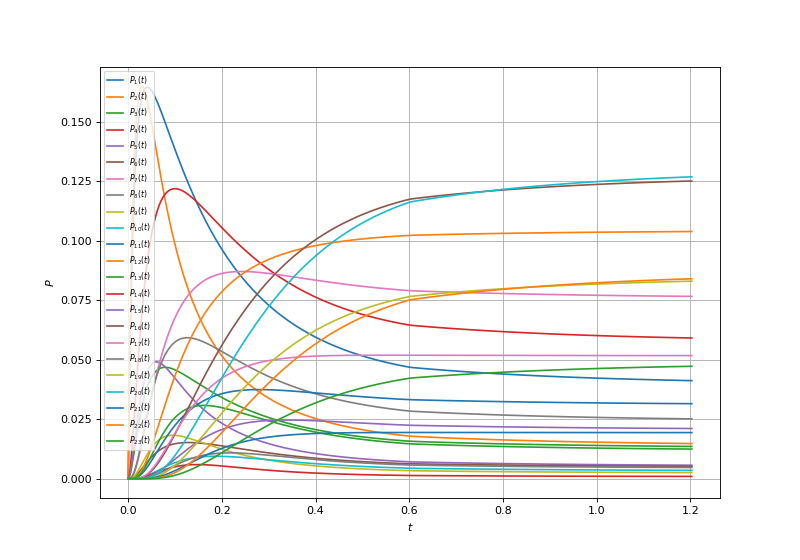
\includegraphics[width=\textwidth]{Images/P_i.png}}
\caption{Функции вероятностей для всех состояний (помимо 0) }
\label{P_i}
\end{figure}

\subsubsection{Прикладные характеристики системы}

Функция отказа может быть определена следующим образом:
$$1-R(t) = P_{term}(t)$$

График функции отказа $1-R(t)$ представлен на рисунке \ref{R_t}.
\begin{figure}[H]
\centerline{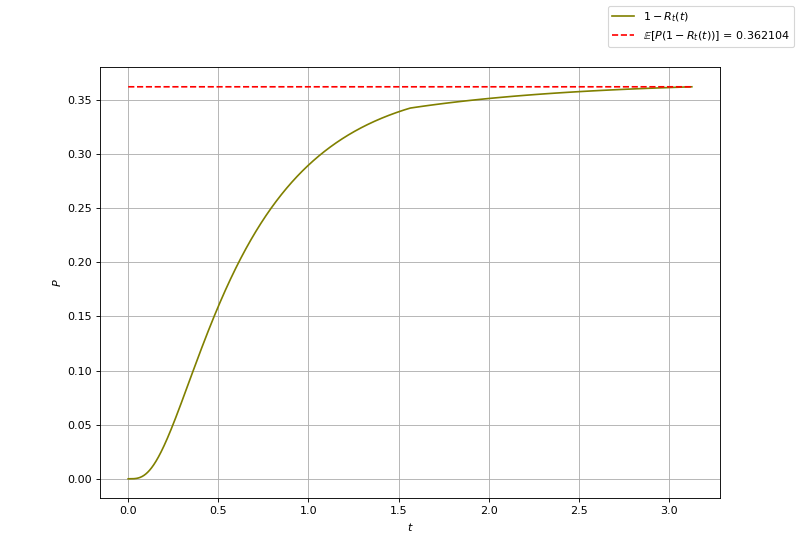
\includegraphics[width=\textwidth]{Images/R_t.png}}
\caption{Функция отказа системы}
\label{R_t}
\end{figure}

\begin{itemize}
    \item Математическое ожидание вероятности отказа:
$\mathbb{E}[P(1-R_t(t))]=0.462682 $;
\item Коэффициент загрузки ремонтной службы: $0.90809$;
\item Среднее число готовых к эксплуатации устройств типа  A и B: $4.26, 3.76$ соответственно;
\end{itemize}

\subsubsection{Имитационное моделирование системы}

Для системы с непрерывным временем была реализована функция, осуществляющая переходы по состояниям.

\begin{lstlisting}[language=python, label=prog,caption={\textit{реализация марковского процесса}}]
# моделирование одного эпизода с непрерывным временем
def MD(m):
    current_s = 0
    current_t = 0
    states_tr = [current_s]
    t_tr = [0]
    times = np.zeros(len(m))
    last = np.zeros(len(m))

    while 1:
        l_b, l_a, l_s = find_lambda(m[current_s])
         # -log(1-y)/(lambda_a+lambda_b)
        t_cur_s = F_t(l_a[0] + l_b[0] + l_s[0],
                      np.random.uniform(low=0.0, high=1.0, size=None))

        times[current_s] += t_cur_s
        current_t += t_cur_s
        idx_b = l_b[1]
        idx_a = l_a[1]
        idx_s = l_s[1]
        current_s = np.random.choice([idx_a, idx_b, idx_s],
                                     p=[l_a[0] / (l_a[0] + l_b[0] + l_s[0]),
                                        l_b[0] / (l_a[0] + l_b[0] + l_s[0]),
                                        l_s[0] / (l_a[0] + l_b[0] + l_s[0])])
        # для дальнейшей отрисовки
        states_tr.append(current_s)
        t_tr.append(current_t)

        if distance.euclidean(times / current_t, last)<0.00001:
            return states_tr, t_tr, [np.mean(w_A), np.mean(w_B)], times / current_t, current_t

        last = times / current_t
\end{lstlisting}



На рисунке \ref{MDP} представлен график переключению состояний системы для 1 прогона ($N=1$).
\begin{figure}[H]
\centerline{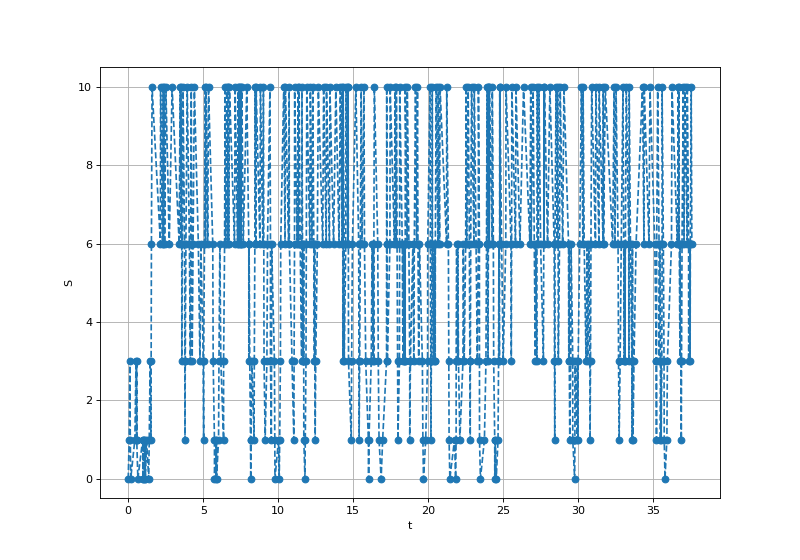
\includegraphics[width=\textwidth]{Images/term.png}}
\caption{График переключению состояний системы}
\label{MDP}
\end{figure}

Для $N=100$:
\begin{itemize}
    \item Среднее $t$ выхода на установившийся режим работы $6.263742156319151$;

    \item Статистические оценки предельных вероятностей после выхода на установившийся режим:
    \[
    \resizebox{\textwidth}{!}{$
[0.39, 0.22, 0.14, 0.12, 0.08, 0.0, 0.04, 0.0, 0.0, 0.0, 0.0, 0.0, 0.0, 0.0, 0.0, 0.0, 0.0]
     $}
\]

\end{itemize}

\subsection{Дискретно-событийное моделирование системы}

Основные элементы дискретно-событийного моделирования системы:
\begin{itemize}
    \item Часы -- текущее "время" внутри моделирования.
    \item События -- поломка или починка устройства.
\end{itemize}
Блок-схема алгортима дискретно-событийного моделирования представлена на рисунке \ref{BS}

\begin{figure}[H]
\centerline{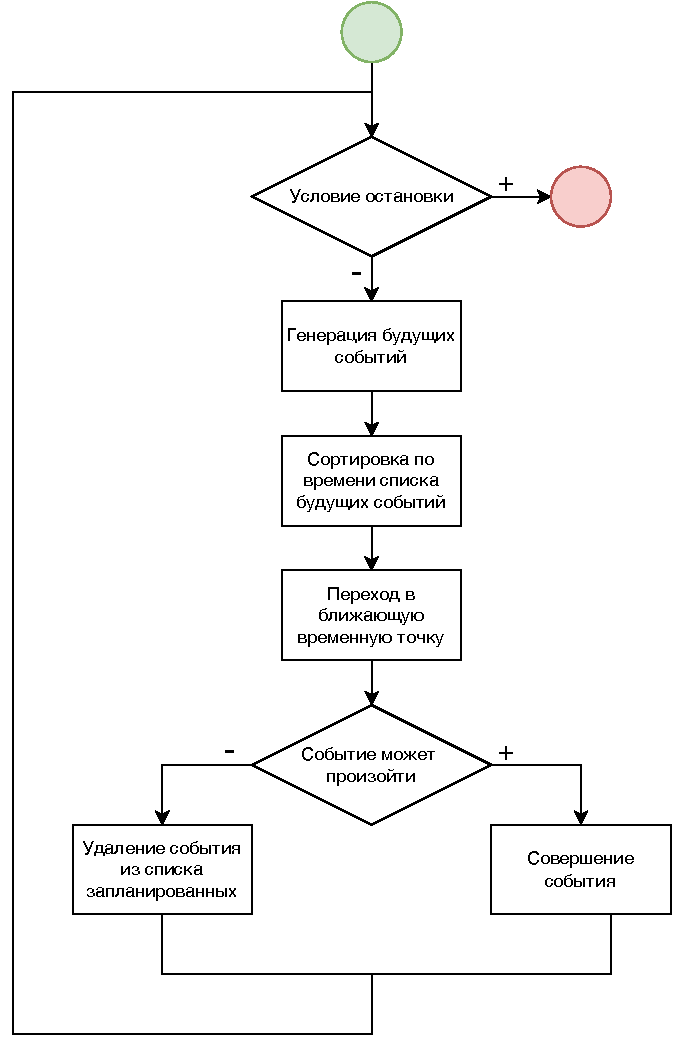
\includegraphics[width=0.5\textwidth]{Images/BS.pdf}}
\caption{Блок-схема алгоритма дискретно-событийного моделирования}
\label{BS}
\end{figure}

Результаты моделирования при $N=1$:
\scriptsize
\begin{verbatim}
Сломан A в момент времени 0.066 всего устройств типа А и В 5 4
                                                  --------------> 4 4
Сломан A в момент времени 0.067 всего устройств типа А и В 4 4
                                                  --------------> 3 4
Сломан B в момент времени 0.082 всего устройств типа А и В 3 4
                                                  --------------> 3 3
Починен A в момент времени 0.095 всего устройств типа А и В 3 3
                                                  --------------> 4 3
Сломан B в момент времени 0.106 всего устройств типа А и В 4 3
                                                  --------------> пропуск события ввиду неработоспособности системы
Сломан B в момент времени 0.126 всего устройств типа А и В 4 3
                                                  --------------> пропуск события ввиду неработоспособности системы
Сломан B в момент времени 0.151 всего устройств типа А и В 4 3
                                                  --------------> пропуск события ввиду неработоспособности системы
Починен A в момент времени 0.166 всего устройств типа А и В 4 3
                                                  --------------> 5 3
Сломан A в момент времени 0.168 всего устройств типа А и В 5 3
                                                  --------------> 4 3
Сломан B в момент времени 0.178 всего устройств типа А и В 4 3
                                                  --------------> пропуск события ввиду неработоспособности системы
Починен A в момент времени 0.208 всего устройств типа А и В 4 3
                                                  --------------> 5 3
Сломан A в момент времени 0.225 всего устройств типа А и В 5 3
                                                  --------------> 4 3
Починен A в момент времени 0.229 всего устройств типа А и В 4 3
                                                  --------------> 5 3
Сломан A в момент времени 0.231 всего устройств типа А и В 5 3
                                                  --------------> 4 3
Сломан A в момент времени 0.238 всего устройств типа А и В 4 3
                                                  --------------> 3 3
Починен A в момент времени 0.239 всего устройств типа А и В 3 3
                                                  --------------> 4 3
Сломан A в момент времени 0.273 всего устройств типа А и В 4 3
                                                  --------------> 3 3
Сломан B в момент времени 0.277 всего устройств типа А и В 3 3
                                                  --------------> пропуск события ввиду неработоспособности системы
Сломан B в момент времени 0.311 всего устройств типа А и В 3 3
                                                  --------------> пропуск события ввиду неработоспособности системы
Сломан A в момент времени 0.319 всего устройств типа А и В 3 3
                                                  --------------> 2 3
Починен B в момент времени 0.332 всего устройств типа А и В 2 3
                                                  --------------> 2 4
Сломан B в момент времени 0.335 всего устройств типа А и В 2 4
                                                  --------------> 2 3
Сломан A в момент времени 0.339 всего устройств типа А и В 2 3
                                                  --------------> 1 3
Сломан A в момент времени 0.341 всего устройств типа А и В 1 3
                                                  --------------> пропуск события ввиду неработоспособности системы
Починен B в момент времени 0.378 всего устройств типа А и В 1 3
                                                  --------------> 1 4
Сломан B в момент времени 0.395 всего устройств типа А и В 1 4
                                                  --------------> 1 3
Сломан B в момент времени 0.405 всего устройств типа А и В 1 3
                                                  --------------> пропуск события ввиду неработоспособности системы
Починен A в момент времени 0.434 всего устройств типа А и В 1 3
                                                  --------------> 2 3
Сломан B в момент времени 0.438 всего устройств типа А и В 2 3
                                                  --------------> пропуск события ввиду неработоспособности системы
Починен A в момент времени 0.441 всего устройств типа А и В 2 3
                                                  --------------> 3 3
Сломан A в момент времени 0.457 всего устройств типа А и В 3 3
                                                  --------------> 2 3
Сломан A в момент времени 0.480 всего устройств типа А и В 2 3
                                                  --------------> 1 3
Сломан B в момент времени 0.490 всего устройств типа А и В 1 3
                                                  --------------> пропуск события ввиду неработоспособности системы
Починен A в момент времени 0.544 всего устройств типа А и В 1 3
                                                  --------------> 2 3
Сломан A в момент времени 0.545 всего устройств типа А и В 2 3
                                                  --------------> 1 3
Починен B в момент времени 0.557 всего устройств типа А и В 1 3
                                                  --------------> 1 4
Сломан A в момент времени 0.563 всего устройств типа А и В 1 4
                                                  --------------> пропуск события ввиду неработоспособности системы
Починен A в момент времени 0.629 всего устройств типа А и В 1 4
                                                  --------------> 2 4
Сломан B в момент времени 0.629 всего устройств типа А и В 2 4
                                                  --------------> 2 3
Сломан B в момент времени 0.629 всего устройств типа А и В 2 3
                                                  --------------> пропуск события ввиду неработоспособности системы
Сломан B в момент времени 0.671 всего устройств типа А и В 2 3
                                                  --------------> пропуск события ввиду неработоспособности системы
Сломан A в момент времени 0.698 всего устройств типа А и В 2 3
                                                  --------------> 1 3
Сломан A в момент времени 0.704 всего устройств типа А и В 1 3
                                                  --------------> пропуск события ввиду неработоспособности системы
Сломан A в момент времени 0.732 всего устройств типа А и В 1 3
                                                  --------------> пропуск события ввиду неработоспособности системы
Починен B в момент времени 0.754 всего устройств типа А и В 1 3
                                                  --------------> 1 4
Сломан B в момент времени 0.764 всего устройств типа А и В 1 4
                                                  --------------> 1 3
Сломан B в момент времени 0.822 всего устройств типа А и В 1 3
                                                  --------------> пропуск события ввиду неработоспособности системы
Сломан B в момент времени 0.865 всего устройств типа А и В 1 3
                                                  --------------> пропуск события ввиду неработоспособности системы
Сломан A в момент времени 0.873 всего устройств типа А и В 1 3
                                                  --------------> пропуск события ввиду неработоспособности системы
Починен A в момент времени 0.898 всего устройств типа А и В 1 3
                                                  --------------> 2 3
Сломан A в момент времени 0.911 всего устройств типа А и В 2 3
                                                  --------------> 1 3
Сломан B в момент времени 0.913 всего устройств типа А и В 1 3
                                                  --------------> пропуск события ввиду неработоспособности системы
Сломан B в момент времени 0.942 всего устройств типа А и В 1 3
                                                  --------------> пропуск события ввиду неработоспособности системы
Сломан A в момент времени 1.029 всего устройств типа А и В 1 3
                                                  --------------> пропуск события ввиду неработоспособности системы
Починен A в момент времени 1.048 всего устройств типа А и В 1 3
                                                  --------------> 2 3
Починен A в момент времени 1.050 всего устройств типа А и В 2 3
                                                  --------------> 3 3
Сломан B в момент времени 1.072 всего устройств типа А и В 3 3
                                                  --------------> пропуск события ввиду неработоспособности системы
Починен B в момент времени 1.084 всего устройств типа А и В 3 3
                                                  --------------> 3 4
Сломан A в момент времени 1.113 всего устройств типа А и В 3 4
                                                  --------------> 2 4
Сломан A в момент времени 1.174 всего устройств типа А и В 2 4
                                                  --------------> 1 4
Сломан A в момент времени 1.213 всего устройств типа А и В 1 4
                                                  --------------> пропуск события ввиду неработоспособности системы
Починен B в момент времени 1.219 всего устройств типа А и В 1 4
                                                  --------------> пропуск события ввиду исправности всех устройств типа В
Починен A в момент времени 1.221 всего устройств типа А и В 1 4
                                                  --------------> 2 4
Починен A в момент времени 1.230 всего устройств типа А и В 2 4
                                                  --------------> 3 4
Сломан A в момент времени 1.231 всего устройств типа А и В 3 4
                                                  --------------> 2 4
Сломан B в момент времени 1.259 всего устройств типа А и В 2 4
                                                  --------------> 2 3
Сломан B в момент времени 1.269 всего устройств типа А и В 2 3
                                                  --------------> пропуск события ввиду неработоспособности системы
Сломан B в момент времени 1.300 всего устройств типа А и В 2 3
                                                  --------------> пропуск события ввиду неработоспособности системы
Сломан A в момент времени 1.321 всего устройств типа А и В 2 3
                                                  --------------> 1 3
Починен A в момент времени 1.424 всего устройств типа А и В 1 3
                                                  --------------> 2 3
Починен A в момент времени 1.475 всего устройств типа А и В 2 3
                                                  --------------> 3 3
Сломан A в момент времени 1.482 всего устройств типа А и В 3 3
                                                  --------------> 2 3
Починен A в момент времени 1.522 всего устройств типа А и В 2 3
                                                  --------------> 3 3
Сломан A в момент времени 1.541 всего устройств типа А и В 3 3
                                                  --------------> 2 3
Сломан A в момент времени 1.554 всего устройств типа А и В 2 3
                                                  --------------> 1 3
Починен B в момент времени 1.555 всего устройств типа А и В 1 3
                                                  --------------> 1 4
Сломан B в момент времени 1.582 всего устройств типа А и В 1 4
                                                  --------------> 1 3
Сломан B в момент времени 1.601 всего устройств типа А и В 1 3
                                                  --------------> пропуск события ввиду неработоспособности системы
Сломан A в момент времени 1.640 всего устройств типа А и В 1 3
                                                  --------------> пропуск события ввиду неработоспособности системы
Починен A в момент времени 1.642 всего устройств типа А и В 1 3
                                                  --------------> 2 3
Сломан A в момент времени 1.648 всего устройств типа А и В 2 3
                                                  --------------> 1 3
Починен A в момент времени 1.649 всего устройств типа А и В 1 3
                                                  --------------> 2 3
Сломан A в момент времени 1.654 всего устройств типа А и В 2 3
                                                  --------------> 1 3
Починен B в момент времени 1.670 всего устройств типа А и В 1 3
                                                  --------------> 1 4
Сломан A в момент времени 1.752 всего устройств типа А и В 1 4
                                                  --------------> пропуск события ввиду неработоспособности системы
Сломан B в момент времени 1.809 всего устройств типа А и В 1 4
                                                  --------------> 1 3
Починен A в момент времени 1.882 всего устройств типа А и В 1 3
                                                  --------------> 2 3
Починен A в момент времени 1.885 всего устройств типа А и В 2 3
                                                  --------------> 3 3
Починен B в момент времени 1.891 всего устройств типа А и В 3 3
                                                  --------------> 3 4
Починен A в момент времени 1.892 всего устройств типа А и В 3 4
                                                  --------------> 4 4
Сломан B в момент времени 1.899 всего устройств типа А и В 4 4
                                                  --------------> 4 3
Починен A в момент времени 1.939 всего устройств типа А и В 4 3
                                                  --------------> 5 3
Сломан B в момент времени 1.945 всего устройств типа А и В 5 3
                                                  --------------> пропуск события ввиду неработоспособности системы
Сломан A в момент времени 1.974 всего устройств типа А и В 5 3
                                                  --------------> 4 3
Сломан A в момент времени 2.028 всего устройств типа А и В 4 3
                                                  --------------> 3 3
Сломан B в момент времени 2.047 всего устройств типа А и В 3 3
                                                  --------------> пропуск события ввиду неработоспособности системы
Сломан B в момент времени 2.109 всего устройств типа А и В 3 3
                                                  --------------> пропуск события ввиду неработоспособности системы
Сломан A в момент времени 2.120 всего устройств типа А и В 3 3
                                                  --------------> 2 3
Сломан B в момент времени 2.123 всего устройств типа А и В 2 3
                                                  --------------> пропуск события ввиду неработоспособности системы
Починен A в момент времени 2.142 всего устройств типа А и В 2 3
                                                  --------------> 3 3
Починен B в момент времени 2.158 всего устройств типа А и В 3 3
                                                  --------------> 3 4
Починен A в момент времени 2.164 всего устройств типа А и В 3 4
                                                  --------------> 4 4
Сломан B в момент времени 2.190 всего устройств типа А и В 4 4
                                                  --------------> 4 3
Сломан B в момент времени 2.283 всего устройств типа А и В 4 3
                                                  --------------> пропуск события ввиду неработоспособности системы
Сломан A в момент времени 2.318 всего устройств типа А и В 4 3
                                                  --------------> 3 3
Починен A в момент времени 2.338 всего устройств типа А и В 3 3
                                                  --------------> 4 3
Починен A в момент времени 2.347 всего устройств типа А и В 4 3
                                                  --------------> 5 3
Починен A в момент времени 2.354 всего устройств типа А и В 5 3
                                                  --------------> пропуск события ввиду исправности всех устройств типа А
Починен A в момент времени 2.355 всего устройств типа А и В 5 3
                                                  --------------> пропуск события ввиду исправности всех устройств типа А
Сломан B в момент времени 2.355 всего устройств типа А и В 5 3
                                                  --------------> пропуск события ввиду неработоспособности системы
Починен A в момент времени 2.383 всего устройств типа А и В 5 3
                                                  --------------> пропуск события ввиду исправности всех устройств типа А
Сломан A в момент времени 2.393 всего устройств типа А и В 5 3
                                                  --------------> 4 3
Сломан B в момент времени 2.421 всего устройств типа А и В 4 3
                                                  --------------> пропуск события ввиду неработоспособности системы
Сломан A в момент времени 2.442 всего устройств типа А и В 4 3
                                                  --------------> 3 3
Сломан B в момент времени 2.562 всего устройств типа А и В 3 3
                                                  --------------> пропуск события ввиду неработоспособности системы
Починен A в момент времени 2.581 всего устройств типа А и В 3 3
                                                  --------------> 4 3
Сломан A в момент времени 2.590 всего устройств типа А и В 4 3
                                                  --------------> 3 3
Починен A в момент времени 2.595 всего устройств типа А и В 3 3
                                                  --------------> 4 3
Сломан A в момент времени 2.609 всего устройств типа А и В 4 3
                                                  --------------> 3 3
Починен A в момент времени 2.613 всего устройств типа А и В 3 3
                                                  --------------> 4 3
Починен A в момент времени 2.653 всего устройств типа А и В 4 3
                                                  --------------> 5 3
Починен A в момент времени 2.665 всего устройств типа А и В 5 3
                                                  --------------> пропуск события ввиду исправности всех устройств типа А
Сломан B в момент времени 2.676 всего устройств типа А и В 5 3
                                                  --------------> пропуск события ввиду неработоспособности системы
Починен A в момент времени 2.681 всего устройств типа А и В 5 3
                                                  --------------> пропуск события ввиду исправности всех устройств типа А
Сломан B в момент времени 2.710 всего устройств типа А и В 5 3
                                                  --------------> пропуск события ввиду неработоспособности системы
Починен A в момент времени 2.849 всего устройств типа А и В 5 3
                                                  --------------> пропуск события ввиду исправности всех устройств типа А
Сломан B в момент времени 2.863 всего устройств типа А и В 5 3
                                                  --------------> пропуск события ввиду неработоспособности системы
Починен A в момент времени 2.866 всего устройств типа А и В 5 3
                                                  --------------> пропуск события ввиду исправности всех устройств типа А
Починен A в момент времени 2.876 всего устройств типа А и В 5 3
                                                  --------------> пропуск события ввиду исправности всех устройств типа А
Починен B в момент времени 2.877 всего устройств типа А и В 5 3
                                                  --------------> 5 4
Починен A в момент времени 2.877 всего устройств типа А и В 5 4
                                                  --------------> пропуск события ввиду исправности всех устройств типа А
Починен A в момент времени 2.878 всего устройств типа А и В 5 4
                                                  --------------> пропуск события ввиду исправности всех устройств типа А
Сломан A в момент времени 2.892 всего устройств типа А и В 5 4
                                                  --------------> 4 4
Сломан A в момент времени 2.893 всего устройств типа А и В 4 4
                                                  --------------> 3 4
Починен A в момент времени 2.897 всего устройств типа А и В 3 4
                                                  --------------> 4 4
Сломан B в момент времени 2.899 всего устройств типа А и В 4 4
                                                  --------------> 4 3
Починен A в момент времени 2.911 всего устройств типа А и В 4 3
                                                  --------------> 5 3
Сломан A в момент времени 2.913 всего устройств типа А и В 5 3
                                                  --------------> 4 3
Сломан B в момент времени 2.926 всего устройств типа А и В 4 3
                                                  --------------> пропуск события ввиду неработоспособности системы

\end{verbatim}
\normalsize

Статистические данные при $N=100$:
\begin{itemize}
    \item Cреднее число готовых к эксплуатации устройств типа A и B = $ 3.96, 3.39 $,
    \item Среднее время выхода в установившийся режим работы = $ 2.3868694724754715 $
\end{itemize}
%-------------------------------------------------
\subsection{Вывод}
В ходе выполнения домашнего задания была промоделирована работа СМО в терминах непрерывных марковских цепей,
а также выполнен анализ ее работы.

% --------------------------------------
% Атрибуты задачи
\labattributes{}{}{}{}{студент группы \EduGroup, \Author}{\Year, \Semestr}
%--------------
